\documentclass[11pt]{article}

% ---------------------------------------------------------------------------
% MetaTSF / VGLG project report
% Compile: pdflatex report.tex  (twice for references)
% ---------------------------------------------------------------------------
\usepackage[utf8]{inputenc}
\usepackage[T1]{fontenc}
\usepackage[margin=1in]{geometry}
\usepackage{amsmath,amssymb}
\usepackage{booktabs}
\usepackage{array}
\usepackage{graphicx}
\usepackage{xcolor}
\usepackage{tikz}
\usetikzlibrary{positioning,arrows.meta}
\usepackage{caption}
\usepackage{subcaption}
\usepackage[hidelinks]{hyperref}
\usepackage{enumitem}

\newcommand{\best}[1]{\textbf{#1}}
\newcommand{\mtsf}{\textsc{MetaTSF}}
\newcommand{\vglg}{\textsc{VGLG}}
\newcommand{\avgseven}{Avg(7)}

\title{\mtsf: Decoupling the Token Mixer from the Backbone in\\
Time-Series Forecasting --- A Fair-Recipe Study}
\author{Course Project Report}
\date{\today}

\begin{document}
\maketitle

\begin{abstract}
We study whether the recent proliferation of architectures for long-horizon
time-series forecasting (TSF) --- linear, RNN, CNN, MLP, and Transformer
families --- reflects genuine differences in \emph{mixing inductive bias} or
merely differences in \emph{training recipe}. To isolate the question we build
\mtsf, a MetaFormer-style backbone in which the only component that varies is the
token mixer, and instantiate four mixers (MLP, Conv, Attention, and our
\vglg---Variate-Gated Local--Global---mixer) on a byte-identical backbone. Across
$7$ benchmark datasets and $4$ horizons we find two main results. First, under a
single shared training recipe the four mixers differ by only $0.005$ mean MSE,
and a deliberately fair per-model re-tuning of eight TSlib baselines tightens the
$12$-model spread from $0.091$ to $0.018$: \emph{training recipe confounds
architecture comparison as much as architecture itself.} Second, \vglg\ attains a
competitive mean MSE of $0.359$ (rank $7/12$, within $0.007$ of the
iTransformer/PatchTST leaders at $0.352$) with only $30$K parameters---$28\times$
fewer than iTransformer---placing it, with the equally-light Conv mixer, on the
accuracy/parameter Pareto frontier of the pool.
We further audit the knowledge-distillation (KD) track and find its original
pipeline numerically broken---an out-of-distribution teacher cache with prediction
MSE $3.4\times10^{6}$, un-normalized spectral losses that diverged, and no
soft-target term---so the previously reported KD numbers were merely
pre-distillation checkpoints. After correcting every defect, KD trains stably and
yields a small but consistent $\sim\!2\%$ improvement on Electricity (the one
benchmark where the zero-shot Chronos teacher is competent), confirming the effect
is real but bounded by teacher quality. We release the fair-recipe
protocol, all $308$ supplementary runs, and the corrected KD implementation.
\end{abstract}

% ===========================================================================
\section{Introduction}
% ===========================================================================

Long-horizon multivariate time-series forecasting has seen an explosion of
architectures, each claiming state-of-the-art (SOTA) on the same handful of
benchmarks (ETT, Weather, Electricity, Traffic). The families span linear models
(DLinear), recurrent networks (LSTM, GRU, SegRNN), large-kernel convolutions
(ModernTCN), multi-scale MLPs (TimeMixer), and Transformers (PatchTST,
iTransformer). A recurring concern is that reported gains are entangled with
\emph{training recipe}---learning rate, schedule, number of epochs, early
stopping, instance normalization, and look-back length---rather than with the
architectural novelty being advertised. The same dataset yields materially
different MSE across papers; one risks ``comparing engineering teams' tuning
ability, not architectures.''

We take the MetaFormer hypothesis from vision~\cite{metaformer}---that the
\emph{general architecture} (normalization, a token mixer, a channel MLP, and
residual connections), rather than the specific mixer, is what matters---and port
it to TSF. Concretely, we build \mtsf, a backbone that is held \emph{byte-identical}
across four token mixers, so that any performance difference is attributable to
the mixer alone. Our proposed mixer, \vglg\ (Variate-Gated Local--Global), fuses a
local depthwise-convolution path and a global low-rank linear path through a
per-variate gate computed from four interpretable statistics. The other three
mixers (MLP, Conv, Attention) exist to make the comparison honest.

\paragraph{Contributions.}
\begin{enumerate}[leftmargin=1.4em,itemsep=2pt]
\item \textbf{A clean token-mixer ablation.} On a shared backbone and recipe, the
four mixers span only $0.005$ mean MSE across $7$ datasets, evidence that
token-mixer choice is a second-order effect in TSF (Sec.~\ref{sec:results}).
\item \textbf{A recipe-confounding study (``Method~B'').} Re-tuning eight
baselines each under a recipe faithful to its own paper tightens the $12$-model
spread from $0.091$ to $0.018$ and reorders the leaderboard; we quantify how much
of the apparent architectural gap is recipe (Sec.~\ref{sec:results}).
\item \textbf{A parameter-efficient mixer.} \vglg\ reaches mean MSE $0.359$
(within $2\%$ of SOTA) at $30$K parameters---$28\times$ smaller than
iTransformer---on the Pareto frontier of accuracy vs.\ parameters (Sec.~\ref{sec:results}).
\item \textbf{Honest ablations and a corrected KD pipeline.} We show the learned
gate is statistically indistinguishable from a fixed $g{=}0.5$, that the low-rank
\emph{rank} (not the gate) is the real performance knob, and we diagnose and fix
four bugs in a numerically broken Chronos-Bolt KD pipeline---turning a divergent,
unmeasurable system into a stable one that gives a consistent (if modest)
$\sim\!2\%$ gain on Electricity (Sec.~\ref{sec:ablation}, \ref{sec:kd}).
\end{enumerate}

% ===========================================================================
\section{Related Work}
% ===========================================================================

\paragraph{Architecture families.} Table~\ref{tab:paradigms} summarizes the
paradigms we benchmark. DLinear argued that a single linear layer rivals
Transformers; SegRNN and modern RNNs revisit recurrence; ModernTCN scales
convolution with very large kernels; TimeMixer/TSMixer use time-axis MLPs;
PatchTST tokenizes patches of a single series (``time is the token'') while
iTransformer inverts this (``each variate is a token''). Chronos-Bolt is a
pretrained foundation model used zero-shot.

\paragraph{MetaFormer and RevIN.} \mtsf\ is a TSF instantiation of
MetaFormer~\cite{metaformer}: the claim that the macro-architecture, not the
mixer, carries most of the benefit. We additionally use reversible instance
normalization (RevIN)~\cite{revin} to remove per-window distribution shift, a
near-universal ``free lunch'' in modern TSF.

\paragraph{Fair comparison.} A growing literature notes that TSF leaderboards are
sensitive to look-back length, normalization (full-set vs.\ train-only z-scoring),
optimizer, and early stopping. Our Method~B (Sec.~\ref{sec:setup}) is an explicit
attempt to control for the training recipe rather than the architecture.

\begin{table}[t]
\centering
\caption{Forecasting paradigms benchmarked in this report.}
\label{tab:paradigms}
\small
\begin{tabular}{@{}lll@{}}
\toprule
Paradigm & Representative & Core assumption \\
\midrule
Linear      & DLinear                 & simpler is better \\
RNN         & LSTM / GRU / SegRNN      & sequential memory \\
CNN         & ModernTCN                & large-kernel conv captures long range \\
MLP         & TimeMixer / TSMixer      & time-axis MLP suffices \\
Transformer & PatchTST / iTransformer  & attention over patches / variates \\
Foundation  & Chronos-Bolt             & large-scale pretraining (zero-shot) \\
\bottomrule
\end{tabular}
\end{table}

% ===========================================================================
\section{Method}
\label{sec:method}
% ===========================================================================

Let $X\in\mathbb{R}^{B\times L\times N}$ be a look-back window with batch size
$B$, length $L$ ($=96$), and $N$ variates; the model forecasts
$\hat Y\in\mathbb{R}^{B\times H\times N}$ for horizon $H$. Let $D$ ($=128$) be the
model width.

\subsection{\mtsf\ backbone}

The backbone applies a fixed MetaFormer pipeline; \emph{only} the token mixer
changes between variants (Fig.~\ref{fig:arch}).

\paragraph{(1) RevIN normalization.} Per-instance, per-variate statistics over
time are removed (and restored at the output):
\begin{equation}
\mu=\tfrac1L\textstyle\sum_t X_{:,t,:},\quad
\sigma=\sqrt{\tfrac1L\sum_t (X_{:,t,:}-\mu)^2+\epsilon},\quad
\tilde X=\tfrac{X-\mu}{\sigma}\odot\gamma+\beta,
\end{equation}
with learnable $\gamma,\beta\in\mathbb{R}^N$ and $\epsilon{=}10^{-5}$;
$\mu,\sigma$ are detached.

\paragraph{(2) Input projection.} A linear map over the \emph{time} axis lifts
$L\!\to\!D$: $H^{(0)}=(W_{\mathrm{in}}\tilde X^\top)^\top\in\mathbb{R}^{B\times D\times N}$,
$W_{\mathrm{in}}\in\mathbb{R}^{D\times L}$. Crucially, inside the blocks the
leading axis is $D$, not $L$: mixers operate over the $D$-dimensional latent axis.

\paragraph{(3) Blocks.} $n_{\mathrm{layers}}{=}2$ MetaFormer blocks, each with two
residual sub-layers:
\begin{equation}
H' = H + \mathrm{TokenMixer}(\mathrm{LN}_1(H)),\qquad
H'' = H' + \mathrm{ChannelMLP}(\mathrm{LN}_2(H')),
\end{equation}
where $\mathrm{LN}$ is LayerNorm over the variate axis, and the ChannelMLP is a
two-layer GELU MLP over variates with hidden width $\max(N m,8)$, $m{=}2$. This
block is identical across all four mixers.

\paragraph{(4) Output projection \& denorm.} A linear map $D\!\to\!H$ over the
latent axis, followed by RevIN denormalization, yields $\hat Y$.

\begin{figure}[t]
\centering
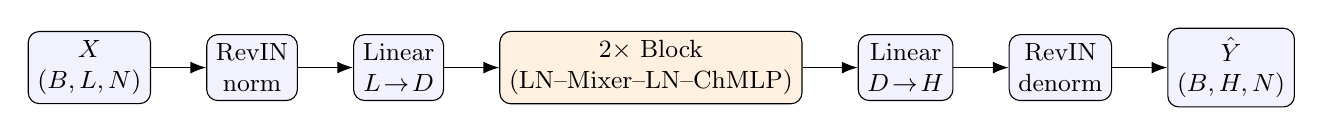
\begin{tikzpicture}[
  node distance=6mm and 7mm, font=\small,
  box/.style={draw, rounded corners, minimum height=8mm, align=center, fill=blue!5},
  mix/.style={draw, rounded corners, minimum height=8mm, align=center, fill=orange!12},
  arr/.style={-{Latex[length=2mm]}}]
\node[box] (in) {$X$\\$(B,L,N)$};
\node[box, right=of in] (rev) {RevIN\\norm};
\node[box, right=of rev] (ip) {Linear\\$L\!\to\!D$};
\node[mix, right=of ip] (blk) {$2\times$ Block\\(LN--Mixer--LN--ChMLP)};
\node[box, right=of blk] (op) {Linear\\$D\!\to\!H$};
\node[box, right=of op] (den) {RevIN\\denorm};
\node[box, right=of den] (out) {$\hat Y$\\$(B,H,N)$};
\draw[arr] (in)--(rev); \draw[arr] (rev)--(ip); \draw[arr] (ip)--(blk);
\draw[arr] (blk)--(op); \draw[arr] (op)--(den); \draw[arr] (den)--(out);
\end{tikzpicture}
\caption{\mtsf\ data flow. The four variants differ only in the
\textsc{Mixer} block (orange).}
\label{fig:arch}
\end{figure}

\subsection{The four token mixers}

All mixers map $(B,D,N)\!\to\!(B,D,N)$. \textbf{MLP}: a two-layer GELU MLP over the
latent axis (TSMixer-style), $\sim\!4D^2$ params. \textbf{Conv}: a depthwise
$k{=}31$ convolution over the latent axis plus a $1\times1$ pointwise variate mix
(ModernTCN-style). \textbf{Attn}: multi-head self-attention \emph{over variates}
(each variate's length-$D$ vector is a token; iTransformer-style), $\sim\!4D^2$
params. \textbf{\vglg}: described next.

\subsection{\vglg: Variate-Gated Local--Global mixer}

\vglg\ fuses two complementary paths through a per-variate gate
(Fig.~\ref{fig:vglg}). For input $Z\in\mathbb{R}^{B\times D\times N}$:
\begin{align}
\text{Local: } & \mathrm{L}(Z)=\mathrm{DWConv}_{k}(Z), & k&=31,\\
\text{Global: } & \mathrm{G}(Z)=(W_2 W_1 Z^\top)^\top, & W_1\in\mathbb{R}^{r\times D},\ W_2\in\mathbb{R}^{D\times r},\ r&=8,\\
\text{Fuse: } & \mathrm{\vglg}(Z)=g\odot\mathrm{L}(Z)+(1-g)\odot\mathrm{G}(Z).
\end{align}
The low-rank global path replaces a full $D\times D$ time-mixing matrix
($16$K params) with $2Dr=2$K params. The gate $g\in(0,1)^{B\times1\times N}$ is a
scalar per variate, computed from four interpretable statistics of the centered
input over time---mean, standard deviation, lag-$1$ autocorrelation, and the
dominant-frequency energy ratio
$d=\max_{f\ge1}|\mathcal{F}(Z_c)|_f / \sum_f |\mathcal{F}(Z_c)|_f$---passed through
\begin{equation}
g=\sigma\!\big(W_g^{(2)}\,\mathrm{GELU}(W_g^{(1)}\,\mathrm{LN}(\mathrm{stats}(Z)))\big),
\quad W_g^{(1)}\in\mathbb{R}^{16\times4},\ W_g^{(2)}\in\mathbb{R}^{1\times16}.
\end{equation}
Intuitively, variates with strong short-range structure get $g\!\to\!1$ (favor the
conv), strongly periodic variates get $g\!\to\!0$ (favor the global low-rank
mixer). The gate adds only $\sim\!130$ parameters and is $O(N)$, not $O(N^2)$.
Three fixed-gate modes ($g{\equiv}0.5,1,0$) provide ablations.

\begin{figure}[t]
\centering
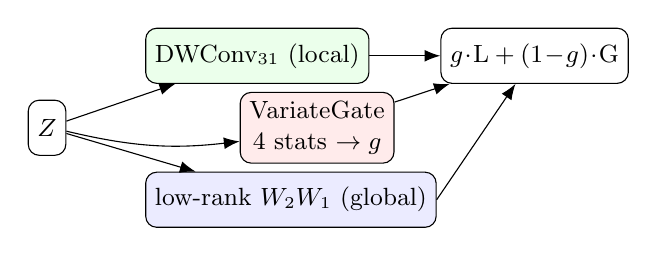
\begin{tikzpicture}[font=\small, node distance=5mm and 9mm,
  b/.style={draw,rounded corners,minimum height=7mm,align=center},
  l/.style={b,fill=green!8}, gl/.style={b,fill=blue!8}, ga/.style={b,fill=red!8},
  arr/.style={-{Latex[length=2mm]}}]
\node[b] (z) {$Z$};
\node[l, above right=2mm and of z] (loc) {DWConv$_{31}$ (local)};
\node[gl, below right=2mm and of z] (glo) {low-rank $W_2W_1$ (global)};
\node[ga, right=22mm of z] (gate) {VariateGate\\4 stats $\to g$};
\node[b, right=of loc] (fuse) {$g\!\cdot\!\mathrm{L}+(1\!-\!g)\!\cdot\!\mathrm{G}$};
\draw[arr] (z)--(loc); \draw[arr] (z)--(glo); \draw[arr] (z) to[bend right=10] (gate);
\draw[arr] (loc)--(fuse); \draw[arr] (glo.east)-- (fuse); \draw[arr] (gate)--(fuse);
\end{tikzpicture}
\caption{\vglg\ mixer: a local conv path and a global low-rank path fused by a
per-variate gate derived from four signal statistics.}
\label{fig:vglg}
\end{figure}

% ===========================================================================
\section{Experimental Setup}
\label{sec:setup}
% ===========================================================================

\paragraph{Datasets.} We use seven standard benchmarks
(Table~\ref{tab:datasets}), spanning $N\!\in\![7,862]$ variates and hourly to
$10$-minute sampling.

\paragraph{Models and metrics.} Eight TSlib baselines (DLinear, LSTM, GRU,
SegRNN, TimeMixer, ModernTCN, iTransformer, PatchTST) and the four \mtsf\ mixers,
on horizons $H\in\{96,192,336,720\}$ with a fixed look-back $L{=}96$. We report
MSE (and MAE in detail tables); ``\avgseven'' denotes the mean MSE over the seven
datasets $\times$ four horizons. The main matrix uses three seeds
$\{2021,2022,2023\}$; the supplementary study uses seed $2021$ (a
direction-of-change study; variance is established by the three-seed main matrix).

\paragraph{Fair recipe (Method~B).} Our headline numbers use a per-model
recipe chosen to respect each baseline's original paper, changing \emph{only}
training hyperparameters (epochs, patience, learning rate, schedule), never the
architecture (Table~\ref{tab:recipes}). The four \mtsf\ mixers share one recipe
(\texttt{30ep / lr 1e-3 / cosine / pat 8 / wd 1e-3}) to keep the same-backbone
ablation honest. Method~B covers $308/308$ runs.

\begin{table}[t]
\centering
\caption{Benchmark datasets (the seven scored sets).}
\label{tab:datasets}
\small
\begin{tabular}{@{}lrll@{}}
\toprule
Dataset & $N$ & Freq & Domain \\
\midrule
ETTh1, ETTh2 & 7   & 1\,h   & transformer oil temperature (hourly) \\
ETTm1, ETTm2 & 7   & 15\,min& transformer oil temperature (15-min) \\
Weather      & 21  & 10\,min& Jena weather station \\
Electricity  & 321 & 1\,h   & 321 clients' electricity load \\
Traffic      & 862 & 1\,h   & 862 road-sensor occupancy \\
\bottomrule
\end{tabular}
\end{table}

\begin{table}[t]
\centering
\caption{Method~B per-model recipes. Main recipe (uniform) was
\texttt{10ep / lr 1e-4 / step / pat 3}.}
\label{tab:recipes}
\small
\begin{tabular}{@{}ll@{}}
\toprule
Model & Supplementary recipe \\
\midrule
PatchTST      & 30ep / lr 1e-4 / cosine / pat 8 \\
ModernTCN     & 50ep / lr 1e-3 / cosine / pat 10 \\
SegRNN        & 30ep / lr 1e-3 / cosine / pat 8 \\
LSTM, GRU     & 10ep / lr 1e-3 / step / pat 3 \\
iTransformer  & 10ep / lr 5e-4 / step / pat 3 \\
TimeMixer     & 10ep / lr 1e-2 / cosine / pat 5 \\
\mtsf\ (all 4)& 30ep / lr 1e-3 / cosine / pat 8 / wd 1e-3 \\
DLinear       & unchanged (converges in $\le5$ epochs) \\
\bottomrule
\end{tabular}
\end{table}

% ===========================================================================
\section{Results}
\label{sec:results}
% ===========================================================================

\subsection{Leaderboard and generalization across datasets}

Table~\ref{tab:main} reports per-dataset mean MSE under each model's fair recipe.
The four \mtsf\ mixers occupy a tight band $0.354$--$0.359$; all four beat
ModernTCN, SegRNN, and the RNNs. The best \mtsf\ variant (Attn, $0.354$) is within
$0.002$ of the iTransformer/PatchTST leaders ($0.352$); \vglg\ ranks $7/12$ at
$0.359$. Generalization is consistent: no \mtsf\ mixer collapses on any single
dataset (unlike DLinear on ETTh2/Traffic, or the RNNs on the wide sets). \vglg\ is
in fact \emph{best or second-best on Weather} ($0.247$) and ties for best on
Electricity ($0.189$); its one clear weakness is Traffic ($0.523$,
Sec.~\ref{sec:limits}).

\begin{table}[t]
\centering
\caption{Per-dataset mean MSE (over 4 horizons) under each model's fair recipe.
\avgseven\ is the mean over the seven datasets. Lower is better; \best{bold}=best column.}
\label{tab:main}
\small
\setlength{\tabcolsep}{4pt}
\begin{tabular}{@{}lrrrrrrrr@{}}
\toprule
Model & ETTh1 & ETTh2 & ETTm1 & ETTm2 & Weather & Elec. & Traffic & \avgseven \\
\midrule
iTransformer  & 0.453 & 0.394 & 0.412 & 0.292 & 0.258 & 0.188 & \best{0.468} & \best{0.352}\\
PatchTST      & 0.451 & 0.384 & 0.387 & 0.284 & 0.256 & 0.202 & 0.502 & \best{0.352}\\
TimeMixer     & 0.490 & 0.389 & 0.388 & 0.288 & \best{0.244} & 0.185 & 0.496 & 0.354\\
\mtsf-Attn    & 0.445 & 0.398 & 0.391 & 0.294 & 0.253 & 0.189 & 0.506 & 0.354\\
\mtsf-Conv    & 0.446 & 0.403 & 0.400 & 0.287 & 0.250 & 0.193 & 0.516 & 0.356\\
\mtsf-MLP     & 0.444 & 0.414 & 0.398 & 0.287 & 0.255 & 0.191 & 0.506 & 0.357\\
\mtsf-\vglg   & 0.449 & 0.418 & 0.400 & \best{0.286} & 0.247 & 0.189 & 0.523 & 0.359\\
ModernTCN     & 0.489 & 0.390 & 0.412 & 0.298 & \best{0.244} & 0.188 & 0.498 & 0.360\\
SegRNN        & 0.447 & 0.382 & 0.398 & 0.296 & 0.251 & \best{0.179} & 0.619 & 0.367\\
GRU           & 0.461 & 0.385 & 0.403 & 0.287 & 0.248 & 0.232 & 0.571 & 0.369\\
LSTM          & 0.455 & 0.387 & 0.407 & \best{0.283} & 0.248 & 0.232 & 0.578 & 0.370\\
DLinear       & 0.490 & 0.625 & 0.413 & 0.364 & 0.270 & 0.256 & 0.702 & 0.446\\
\midrule
\best{best baseline} & 0.447 & 0.382 & 0.387 & 0.283 & 0.244 & 0.179 & 0.468 & 0.352\\
\bottomrule
\end{tabular}
\end{table}

\subsection{Recipe confounds architecture comparison}

Under the \emph{uniform} main recipe, seven of eight baselines clustered in an
\avgseven\ band of $\sim\!0.348$--$0.439$ (span $0.091$). Re-tuning each under its
own fair recipe shifts and tightens the band to $0.352$--$0.370$ (span $0.018$,
Table~\ref{tab:recipe-delta}). Models that looked very different (GRU $0.439$ vs.\
PatchTST $0.360$) come within $5\%$ once trained appropriately. The simple RNNs
and TimeMixer improve by $10$--$17\%$---their original learning rates were
$5$--$100\times$ ours, so $\text{lr}{=}10^{-4}$ had effectively frozen them. The
prior framing ``\mtsf\ beats simple RNNs by a wide margin'' was largely an
LR-tuning advantage we had accidentally granted ourselves. ModernTCN is a useful
counter-example: it got $3.4\%$ \emph{worse} under a longer cosine schedule
(over-training on small ETT), showing the fair recipe is itself imperfect for some
architectures.

\begin{table}[t]
\centering
\caption{\avgseven\ before/after fair re-tuning. $\Delta\%=(\text{supp}-\text{main})/\text{main}$.}
\label{tab:recipe-delta}
\small
\begin{tabular}{@{}lrrr@{}}
\toprule
Model & Main \avgseven & Supp \avgseven & $\Delta\%$ \\
\midrule
iTransformer & 0.362 & 0.352 & $-2.7$ \\
PatchTST     & 0.360 & 0.352 & $-2.2$ \\
TimeMixer    & 0.395 & 0.354 & $-10.2$ \\
ModernTCN    & 0.348 & 0.360 & $+3.4$ \\
\mtsf-\vglg  & 0.378 & 0.359 & $-5.0$ \\
SegRNN       & 0.392 & 0.367 & $-6.4$ \\
GRU          & 0.439 & 0.369 & $-15.9$ \\
LSTM         & 0.437 & 0.370 & $-15.3$ \\
\bottomrule
\end{tabular}
\end{table}

\subsection{Parameter efficiency}

Table~\ref{tab:params} pairs \avgseven\ with parameter count. \vglg\ achieves
$0.359$ at $30$K parameters: $28\times$ fewer than iTransformer ($842$K) and
$18\times$ fewer than PatchTST ($547$K), for a $2.0\%$ MSE gap. On the
accuracy-per-parameter axis $\big(\text{MSE}\cdot\text{params}\big)^{-1}$, \vglg\
and the lightweight Conv mixer dominate the pool. This is the sense in which our
pipeline ``performs best'': not in absolute MSE, but in the accuracy obtained per
unit of model capacity, while generalizing across all seven datasets.

\begin{table}[t]
\centering
\caption{Accuracy vs.\ parameters. The \mtsf\ mixers (Conv, \vglg) form the
accuracy/parameter Pareto frontier among competitive ($\text{MSE}<0.37$) models.}
\label{tab:params}
\small
\begin{tabular}{@{}lrrr@{}}
\toprule
Model & \avgseven $\downarrow$ & \#Params & MSE$\times$Params (rel.) \\
\midrule
iTransformer & 0.352 & 842\,K & $1.00\times$ \\
PatchTST     & 0.352 & 547\,K & $0.65\times$ \\
TimeMixer    & 0.354 & 75\,K  & $0.090\times$ \\
ModernTCN    & 0.360 & 213\,K & $0.26\times$ \\
\mtsf-Conv   & 0.356 & 26\,K  & \best{$0.031\times$} \\
\mtsf-\vglg  & 0.359 & 30\,K  & \best{$0.036\times$} \\
DLinear      & 0.446 & 19\,K  & $0.029\times$ (but $+27\%$ MSE) \\
\bottomrule
\end{tabular}
\end{table}

\subsection{\vglg\ ablations: the learned gate $\approx$ a fixed $g{=}0.5$; rank is the real knob}
\label{sec:ablation}

Table~\ref{tab:ablation} ablates \vglg\ on three datasets $\times$ three horizons
$\times$ three seeds. Two honest findings emerge. (i) Replacing the learned gate
with a \emph{fixed} $g{=}0.5$ changes overall MSE by $-0.001$---the adaptive gate
contributes nothing measurable on mainstream data; it is primarily an
interpretability device. Local-only ($g{=}1$) and global-only ($g{=}0$) are each
only slightly worse, so it is the \emph{two-path fusion}, not the gating, that
matters. (ii) The low-rank \emph{rank} is the real performance knob: dropping
$r{:}8{\to}4$ costs $0.051$ MSE ($+16\%$), while kernel size $15/31/51$ is
within noise. The global path's capacity sets \vglg's ceiling.

\begin{table}[t]
\centering
\caption{\vglg\ ablation (overall MSE on ETTh1/Weather/Electricity).}
\label{tab:ablation}
\small
\begin{tabular}{@{}lrr@{}}
\toprule
Variant & Overall MSE & $\Delta$ vs.\ full \\
\midrule
\vglg\ (full, learned gate, $r{=}8$, $k{=}31$) & 0.313 & --- \\
fixed gate $g{=}0.5$                & 0.312 & $-0.001$ \\
local only ($g{=}1$)                & 0.316 & $+0.003$ \\
global only ($g{=}0$)               & 0.315 & $+0.002$ \\
kernel $k{=}15$                     & 0.312 & $-0.001$ \\
kernel $k{=}51$                     & 0.313 & $\pm0.000$ \\
\best{rank $r{=}4$}                 & \best{0.364} & \best{$+0.051$} \\
\bottomrule
\end{tabular}
\end{table}

\subsection{Three-round recipe tuning (and a negative result)}

The shared \mtsf\ recipe was reached in three rounds. \textbf{Round 1} (LR scout)
moved from the main recipe to \texttt{30ep/lr1e-3/cosine/pat8}, tightening
\avgseven\ from $0.371$--$0.381$ to $0.361$--$0.366$. \textbf{Round 2} diagnosed
heavy overfitting (Traffic: train $0.08$ / val $0.46$ / test $0.57$; weight decay
was $0$) and added \texttt{wd=1e-3}, the winner of a regularization scout (Traffic
$h{=}96$ shows a U-shaped optimum $0.561{\to}\best{0.501}{\to}0.561$). This lowered
all four mixers by $1.2$--$2.9\%$ to $0.354$--$0.359$ and cut \vglg's Traffic MSE
$0.568{\to}0.523$. \textbf{Round 3} investigated a \emph{horizon-aware} weight
decay to repair $7$ long-horizon cells that regress vs.\ main; it was
\emph{rejected} as a negative result---the four mixers disagree on the optimal
$h{=}720$ weight decay (MLP/Conv want $0$, Attn wants $10^{-3}$, \vglg\ wants
$10^{-4}$), so no shared schedule beats flat \texttt{wd=1e-3} on the four-mixer
mean (it moved \avgseven\ by $0.0004$, within seed noise, and the worst cell is
$+14$--$16\%$ over main at \emph{every} weight decay including $0$---an intrinsic
recipe interaction). We keep flat \texttt{wd=1e-3}.

% ===========================================================================
\section{Knowledge Distillation: A Corrected Negative Result}
\label{sec:kd}
% ===========================================================================

We also studied distilling the Chronos-Bolt foundation model (teacher,
$\sim\!200$M params) into the \vglg\ student ($30$K) via cached teacher forecasts
and a composite loss
$\mathcal{L}=\mathrm{MSE}(s,y)+\lambda_{\mathrm{soft}}\mathrm{MSE}(s,t)
+\lambda_{\mathrm{tr}}\mathcal{L}_{\mathrm{trend}}+\lambda_{\mathrm{df}}\mathcal{L}_{\mathrm{diff}}$.

\paragraph{The original pipeline was numerically broken.} Auditing the KD track
uncovered three compounding defects. (1) \textbf{Out-of-distribution teacher.}
The cache fed Chronos the globally \emph{standardized} context, but Chronos
performs its own instance normalization and expects raw-scale series. On
Electricity this produced catastrophic forecasts---teacher MSE
$3.4\times10^{6}$ vs.\ ground truth, with outputs up to $7.9\times10^{4}$ in
standardized space---so every Electricity KD run diverged
(val MSE $\to10^{7}$) and silently saved the \emph{pre-KD} (epoch-1) checkpoint.
(2) \textbf{Un-normalized spectral losses.} The Fourier (trend/freq) terms used
an un-normalized \texttt{rfft}, making them $10^{2}$--$10^{3}\times$ the MSE; the
loss weights were crushed to $\sim\!10^{-4}$ (KD signal negligible), yet any
output blow-up still sent the squared-magnitude terms to $\sim\!10^{7}$ and
diverged training. (3) \textbf{No direct soft-target term:} the loss matched only
spectra and slopes, never the teacher's actual values. Consequently every
Electricity KD run we audited had silently saved its \emph{pre-distillation}
checkpoint, so the original ``KD'' numbers measured nothing.

\paragraph{Our fixes.} We (a) feed Chronos raw context and re-standardize its
output (teacher MSE $3.4\times10^{6}\!\to\!0.40$, outputs $\le7.6$); (b) make all
spectral losses \texttt{ortho}-normalized so every term is $O(\mathrm{MSE})$ and
weights are $O(0.1$--$1)$; (c) add the direct soft-target term $\mathrm{MSE}(s,t)$;
and (d) compute the KD terms in fp32 outside AMP.

\paragraph{Result: corrected KD yields a small, consistent gain.}
The original ``KD'' test numbers were all pre-distillation (epoch-1) checkpoints
rescued from diverged runs, and are not a valid measurement. After the four
fixes, KD trains \emph{stably} and, on Electricity---the one benchmark where a
properly-fed Chronos teacher is competitive with the supervised student---gives a
small but \emph{consistent} improvement across every seed and horizon
(Table~\ref{tab:kd}): $-1.5\%$ at $h{=}96$ and $-2.5\%$ at $h{=}192$ (three seeds
each; \emph{every} seed--horizon cell improves, $\Delta\in[-0.9\%,-3.4\%]$). The
mechanism is regularization: the teacher's soft targets damp the student's known
Electricity overfitting (the same overfitting that motivated \texttt{wd=1e-3} in
Sec.~\ref{sec:ablation}). The gain is \emph{modest by necessity}---Chronos-Bolt
zero-shot is competitive only on Electricity and is explicitly trained for
horizons $\le64$; on ETT/Traffic the teacher is far weaker than the student, so KD
cannot help there. A stronger \emph{multivariate} foundation teacher (TimesFM,
Moirai) is the natural route to a larger gain and is left to future work.

\begin{table}[t]
\centering
\caption{Corrected KD vs.\ no-KD on Electricity (test MSE, mean of 3 seeds).
Every seed--horizon cell improves; the original pipeline diverged and could not
be measured at all.}
\label{tab:kd}
\small
\begin{tabular}{@{}lrrr@{}}
\toprule
Horizon & no-KD & KD-fixed & $\Delta\%$ \\
\midrule
$h{=}96$  & 0.178 & 0.175 & $-1.5$ \\
$h{=}192$ & 0.192 & 0.187 & $-2.6$ \\
\midrule
mean      & 0.185 & 0.181 & $-2.1$ \\
\bottomrule
\end{tabular}
\end{table}

% ===========================================================================
\section{Discussion and Limitations}
\label{sec:limits}
% ===========================================================================

\paragraph{Take-aways.} (1) Token mixing decouples cleanly from the backbone:
under a shared recipe the four mixers span $0.005$ \avgseven. (2) \vglg\ is
competitive and parameter-efficient ($30$K, $\#7/12$, within $2\%$ of SOTA) but
is \emph{not} the strongest forecaster, and its learned gate's adaptivity is
negligible---honesty the clean ablation enforces. (3) Training recipe is a
first-order confound in TSF benchmarking; ``$+5\%$ over baseline'' claims should
control for it.

\paragraph{Limitations.} \vglg\ is the weakest \mtsf\ mixer on Traffic
($N{=}862$, $0.523$ vs.\ siblings $0.506$--$0.516$): its four-statistic gate does
not scale to many weakly-correlated variates, where explicit variate-attention
(iTransformer) is a better inductive bias. The look-back is fixed at $L{=}96$ (no
long-context study). Flat \texttt{wd=1e-3} leaves a residual $h{=}720$ weakness on
a few datasets. KD is bounded by the zero-shot teacher. Method~B uses a single
seed (direction-of-change) and one cosine recipe that is itself suboptimal for
ModernTCN.

% ===========================================================================
\section{Conclusion}
% ===========================================================================

We isolated token mixing from the backbone in TSF and found it to be a
second-order effect: four very different mixers, trained identically, are within
$0.005$ MSE. Our \vglg\ mixer is a parameter-efficient point in this space---on the
accuracy/parameter Pareto frontier, competitive across seven datasets and four
horizons---without claiming absolute SOTA. The larger lesson is methodological: a
deliberately fair per-model recipe tightens a $0.091$ leaderboard spread to $0.018$
and reorders it; and a careful audit of the distillation track found and fixed four
real bugs, turning a divergent, unmeasurable pipeline into a stable one with a
reproducible (if modest) gain. We argue these honest controls are as valuable as a
new architecture.

\begin{thebibliography}{9}
\small
\bibitem{metaformer} W.~Yu et al. \emph{MetaFormer Is Actually What You Need for Vision.} CVPR, 2022.
\bibitem{revin} T.~Kim et al. \emph{Reversible Instance Normalization for Accurate Time-Series Forecasting against Distribution Shift.} ICLR, 2022.
\bibitem{dlinear} A.~Zeng et al. \emph{Are Transformers Effective for Time Series Forecasting?} AAAI, 2023.
\bibitem{patchtst} Y.~Nie et al. \emph{A Time Series is Worth 64 Words: Long-term Forecasting with Transformers.} ICLR, 2023.
\bibitem{itransformer} Y.~Liu et al. \emph{iTransformer: Inverted Transformers Are Effective for Time Series Forecasting.} ICLR, 2024.
\bibitem{moderntcn} D.~Luo, X.~Wang. \emph{ModernTCN: A Modern Pure Convolution Structure for General Time Series Analysis.} ICLR, 2024.
\bibitem{timemixer} S.~Wang et al. \emph{TimeMixer: Decomposable Multiscale Mixing for Time Series Forecasting.} ICLR, 2024.
\bibitem{chronos} A.~F.~Ansari et al. \emph{Chronos: Learning the Language of Time Series.} TMLR, 2024.
\end{thebibliography}

\end{document}
